

% ------------- Informe de Analogicas ----------------%


\documentclass{article}
%-------------- Declaracion de Paquetes --------------%
\usepackage[T1]{fontenc}						% No me acuerdo para que era este paquete jejeje
\usepackage[spanish]{babel}					% paquete para poner cosas en español
\usepackage{titling}								% paquete para modificar el espaciado de los titulos
\usepackage[a4paper,margin=1in]{geometry}	% paquete para poner márgenes más pequeños
\usepackage{titlesec}							% paquete para modificar como se ven los titulos
\usepackage{graphicx}							% paquete para meter imagenes
\usepackage{todonotes}							% paquete para hacer \todo
\usepackage{hyperref}							% paquete para hacer hyperreferencias a links
\usepackage{minted}								% paquete para meter codigo
\usepackage{float}								% paquete para poder usar \begin {figure}[H]
\usepackage{wrapfig}								% paquete para hacer wrapfigure
\usepackage{pdfpages}							% paquete para incluir pdfs
\usepackage{tikz}									% paquete para meter un borde en el margen
\usepackage{amsmath}								% paquete con cosas de matematicas
\usepackage{amsfonts}							% idem
\usepackage{amssymb} 							% idem
\usepackage{bm}									% paquete para poder hacer bold en matematicas
\usepackage{enumitem}							% paquete para hacer enumeracion con a b c
\usepackage{xurl}									% paquete para tener linewrap en las url
\usepackage{fancyhdr}							% paquete para hacer \cfoot{\thepage}
\usepackage{soulutf8}							% paquete para poder hacer \ul
\usepackage{subfiles}
\usepackage{blindtext}

%------------------- Configuracion -------------------%

%Estas 3 lineas activan el modo oscuro en el pdf, es hermoso:
%\usepackage{xcolor}
%\pagecolor[rgb]{0,0,0} %black
%\color[rgb]{1,1,1} %white
\hypersetup{								% Setup of hyperref package
	 colorlinks=true,
	 linkcolor=black,			%modo claro
	 %linkcolor=white,		%modo oscuro
	 filecolor=brown,		
	 urlcolor=blue,
	 pdftitle={Informe Analogica},
	 }
\graphicspath{{imagenes/}}
\setcounter{tocdepth}{3}

\newcommand{\vc}{\overrightarrow}
\newcommand{\x}{\cdot}

\pagestyle{fancy}
\rhead{Informe Técnico}
\rfoot{Página \thepage}
\cfoot{}
\renewcommand{\headrulewidth}{2pt}
\renewcommand{\footrulewidth}{1pt}
%-------------- Formatos de los titulos --------------%

\newcommand{\sectionbreak}{\clearpage}
\newcommand{\subsectionbreak}{\clearpage}

\titleformat{\section}
	{\bfseries \huge}
	{}
	{0em}
	{}[\titlerule]

\titleformat{\subsection}
	{\bfseries \Large \centering}
	{}
	{0em}
	{}

\titleformat{\subsubsection}
	{\bfseries \large}
	{}
	{0em}
	{\ul}

\titlespacing{\section} %me permite controlar el espaciado de la seccion que le indico
	{0em}
	{0em}
	{1.5em}

\titlespacing{\subsection}
{0em} %sangria
{3em} %separacion con lo que hay arriba
{1em} %separacion con lo que hay abajo

%-----------------------------------------------------%
%--------------- Inicio del documento ----------------%

\begin{document}
% Para meter un borde de pagina en cada página
% \usetikzlibrary{calc}
% \SetBgScale{1}
% \SetBgAngle{0}
% \SetBgColor{black}
% \SetBgOpacity{0.7}
% \SetBgContents{
% \begin{tikzpicture}[overlay,remember picture]
% \draw [line width=1.5pt]
%     ($ (current page.north west) + (0.8in,-0.8in) $)
%     rectangle
%     ($ (current page.south east) + (-0.8in,0.8in) $);
% \end{tikzpicture}}
%--------------- Inicio del titulo -------------------%
\begin{titlepage}
	\begin{center}
		\vspace{1cm}

		{\Huge
		\textbf{Informe técnico final}}

		\vspace{0.5cm}
		{\Large
		Un trabajo presentado para la materia de \\
		Aplicaciones de Electronica Analógica}
				
		\vspace{0.5cm}
		\begin{figure}[H]
			\centering
			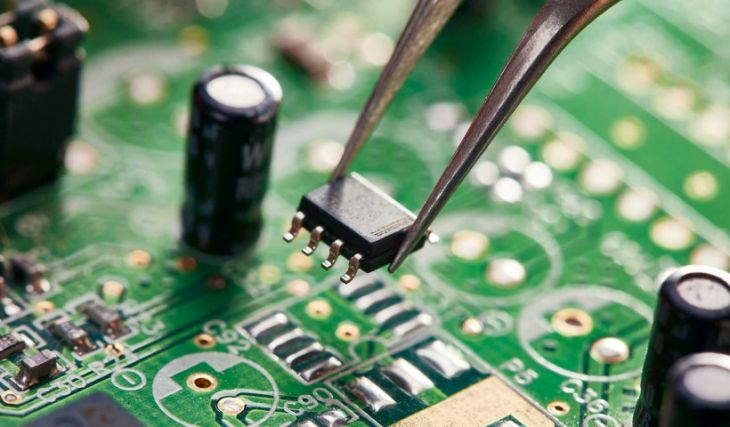
\includegraphics[width=0.6\textwidth]{logo.jpeg}
		\end{figure}
		
		\vfill
	
	\end{center}
	\subsubsection{Integrantes:}
	\begin{itemize}
		\item	Baccheto, Hernan
		\item	Borea, Santiago
		\item	Fariña, Francisco
		\item	Fernandez, Malenotti Maximo
		\item	Fink, Maximo
		\item	Golmar, Elias
		\item	Krapp, Ramiro
		\item	Lopez, Yamir
		\item	Perez, Thomas
		\item	Pisacane, Juan Cruz
		\item	Roldan, Jeremias
		\item	Sacchi, Octavio
		\item	Trostch, Demian
		\item	Volpatti, Luca
		\item	Wendler, Tomás
	\end{itemize}
	
	\vfill{}

	\begin{center}
		{\Large
			Instituto tecnológico San Bonifacio\\
			Departamento de electrónica\\
			\today
		}
		
		\vspace{0.5cm}
		{\large Hecho en \LaTeX\\
		Versión 1.0}\\
	\end{center}
\end{titlepage}

\tableofcontents		\noindent\rule{\textwidth}{0.7pt}
\\ El índice tiene hipervínculos incorporados!\\ 
Toca en cada seccion y automaticamente tu lector de pdfs te llevara a esa página\\\\

%\listoftodos		%Borrar esto para el documento final!!! FLAG


{
\titleformat{\subsubsection}
	{\large}
	{}
	{0em}
	{\ul}

\titlespacing{\subsubsection}
{0em} %sangria
{1.5em} %separacion con lo que hay arriba
{0.4em} %separacion con lo que hay abajo


	\section{Division de Temas}
		\subsubsection{Armado del Documento y pasado a {\LaTeX}}
		\begin{itemize}
			\item Krapp, Ramiro
		\end{itemize}

		\subsubsection{Grafico Lineal y Logarítmico}
		\begin{itemize}
			\item Santiago, Borea
		\end{itemize}

		\subsubsection{Amplificadores Operaciones}
		\begin{itemize}
			\item Golmar, Elias	
		\end{itemize}

		\subsubsection{Cuadripolos}
		\begin{itemize}
			\item Fernandez Malenotti, Maximo
			\item Baccheto, Hernan
		\end{itemize}

		\subsubsection{Compensación de Perdida de Potencia}
		\begin{itemize}
			\item Pisacane, Juan Cruz
			\item Trosch, Demian
			\item Fink, Máximo
			\item Lopez, Yamir
			\item Fariña, Francisco
		\end{itemize}

		\subsubsection{Analisis de Fourier}
		\begin{itemize}
			\item Volpatti, Luca
		\end{itemize}

		\subsubsection{Applet de Fourier}
		\begin{itemize}
			\item Roldan Jeremías
			\item Wendler, Tomas
		\end{itemize}

		\subsubsection{Filtros}
		\begin{itemize}
			\item Krapp Ramiro
			\item Sacchi, Octavio
			\item Perez, Thomas
		\end{itemize}

		\subsubsection{Código G}
		\begin{itemize}
			\item Krapp, Ramiro
			\item Perez, Thomas
		\end{itemize}

}

{
	\lfoot{Borea, Santiago }
	\subfile{subfiles/grafico-lin-log.tex}
	\clearpage
}

{
	\lfoot{Golmar, Elias}
	\subfile{subfiles/opamp.tex}
	\clearpage
}

{
	\lfoot{Bachetto, Hernan --- Malenotti, Máximo}
	\subfile{subfiles/cuadripolos.tex}
	\clearpage
}

{
	\lfoot{Pisacane J.C. --- Fink M. --- Trosch D. --- Lopez Y. --- Fariña F.}
	\subfile{subfiles/potencia.tex}
	\clearpage
	
}	

{
	\lfoot{Volpatti, Luca}
	\subfile{subfiles/fourier.tex}
	\clearpage
}
{
	\lfoot{Roldan, Jeremías --- Wendler, Tomás}
	\subfile{subfiles/applet.tex}
	\clearpage
}

{
	\lfoot{Krapp Ramiro --- Perez, Thomas --- Sacchi, Octavio}
	\subfile{subfiles/filtros.tex}
	\clearpage
}

{
	\lfoot{Krapp, Ramiro --- Perez, Thomas}
	\subfile{subfiles/codigoG.tex}
	\clearpage
}

\section{Bibliografía y Referencias}
\begin{itemize}
	\item \url{https://laboratoriolinux.es/index.php/-noticias-mundo-linux-/
		aula-linuxera/aula/16225-filtros-paso-bajo-paso-alto-paso-de-todo-me-piro-de-aqui.html}
	
	\item \url{https://www.electrical4u.com/cutoff-frequency/}
	
	\item Lecture Notes for EE 261 --- The Fourier Transform and its Applications\\
		Prof. Brad Osgood\\
		Electrical Engineering Department\\
		Stanford University              
	
	\item Introducción a la teoría y sistemas de comunicación                   \\
		Prof. B. P. Lathi   

	\item Fourier Analysis \\
		Prof. T.W Körner    \\
		Cambridge University
	\item \url{https://spa.answersexpress.com/single-ended-differential-amplifiers-48264}
\end{itemize}
\end{document}
